\problemname{Monopol}
Jocke och hans vänner brukar spela Monopol med varandra.
Efter otaliga spel har de tröttnat på de vanliga reglerna, och har därför ändrat på dem en aning.

Först väljer de ett lagom stort land.
De tar sedan en titt på vägnätet i landet och väljer ut en sekvens av \textbf{olika} städer $v_1, v_2, \dots, v_k$ som bildar en \emph{cykel}.
Detta innebär att det finns en direkt väg mellan städerna $v_i$ och $v_{i+1}$ för alla $1 \le i < k$ samt $v_k$ och $v_1$, precis som på ett monopolbräde.
Därefter åker de till landet, och spelar genom att åka runt cykeln i sina bilar för att köpa och sälja fastigheter med riktiga pengar.

Det finns dock en begränsning som gör det svårt att genomföra spelet: de måste hitta en lämplig cykel i vägnätet.
Vissa länder har nämligen ett väldigt stora vägnät.
Något som försvårar ytterligare är att cykeln måste ha ett jämnt antal vägar, för annars funkar inte reglerna (``Fri parkering'' hamnar inte
i mitten vilket ger ett obalanserat spel).

Givet landets alla städer samt mellan vilka par av städer det går vägar, hitta en cykel som består av ett jämnt antal vägar om det finns en.

\begin{figure}[!h]
  \centering
  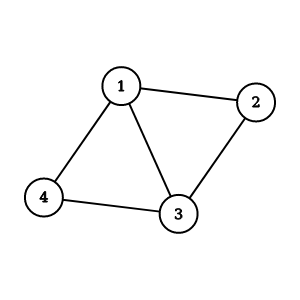
\includegraphics[width=5cm]{sample1.png}
  \quad
  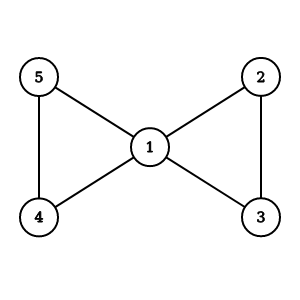
\includegraphics[width=5cm]{sample2.png}
  \quad
  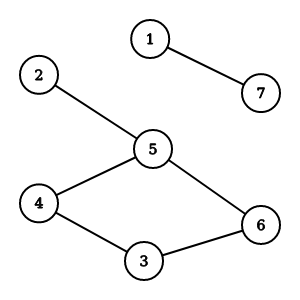
\includegraphics[width=5cm]{sample3.png}
  \caption{Illustration av länderna i de tre exempelfallen.}
\end{figure}

\section*{Indata}
Den första raden innehåller de två heltalen $N$ ($1 \le N \le 10^5$) och $M$ ($0 \le M \le \min(2 \cdot 10^5, \frac{n(n-1)}{2}$), antalet städer respektive antalet vägar som vägnätet består av.

Sedan följer $M$ rader med två heltal $a$ och $b$ vardera, vilket betyder att det finns en väg mellan städerna $a$ och $b$ i landet ($1\le a \neq b \le N$).
Det är garanterat att det inte finns flera vägar mellan samma par av städer i landet.

\section*{Utdata}
Om det inte finns en jämn cykel, skriv ut en rad med strängen ``\texttt{NO}''.

Om det finns en jämn cykel, skriv ut en rad med strängen ``\texttt{YES}''.
Därefter ska du skriva ut en sådan cykel.
Skriv först ut en rad med ett \textbf{jämnt} heltal $k$ ($4\le k \le N$), antalet städer i din cykel.
På nästa rad, skriv ut $k$ stycken \textbf{olika} heltal $v_{1}, v_{2}, \ldots, v_{k}$ ($1\le v_{i}\le N$) separerade av blanksteg: städerna i din cykel.
Det måste gälla att det finns vägar mellan städerna $(v_{1},v_{2}), (v_{2},v_{3}),\ \ldots, (v_{k-1},v_{k}), (v_{k}, v_{1})$.

Om det finns flera möjliga cykler kan du skriva ut vilken som helst.

\section*{Poängsättning}
Din lösning kommer att testas på en mängd testfallsgrupper.
För att få poäng för en grupp så måste du klara alla testfall i gruppen.

\noindent
\begin{tabular}{| l | l | l |}
  \hline
  Grupp & Poängvärde & Gränser \\ \hline
  $1$ & 18 & $N\le 10$ \\ \hline
  $2$ & 16 & $N\le 100$ och $M\le 200$ \\ \hline
  $3$  & 17 & Städerna kan delas in i två delar så att ingen väg går mellan två städer i samma del \\ \hline
  $4$  & 13 & Alla städer i landet har en direkt väg till högst 2 städer \\ \hline
  $5$  & 20 & Alla städer i landet har en direkt väg till högst 3 städer \\ \hline
  $6$  & 16 & Inga ytterligare begränsningar \\ \hline
\end{tabular}
